\documentclass[journal]{IEEEtran}
\usepackage[a5paper, margin=10mm, onecolumn]{geometry}
%\usepackage{lmodern} % Ensure lmodern is loaded for pdflatex
\usepackage{tfrupee} % Include tfrupee package

\setlength{\headheight}{1cm} % Set the height of the header box
\setlength{\headsep}{0mm}     % Set the distance between the header box and the top of the text

\usepackage{gvv-book}
\usepackage{gvv}
\usepackage{cite}
\usepackage{amsmath,amssymb,amsfonts,amsthm}
\usepackage{algorithmic}
\usepackage{graphicx}
\usepackage{textcomp}
\usepackage{xcolor}
\usepackage{txfonts}
\usepackage{listings}
\usepackage{enumitem}
\usepackage{mathtools}
\usepackage{gensymb}
\usepackage{comment}
\usepackage[breaklinks=true]{hyperref}
\usepackage{tkz-euclide} 
\usepackage{listings}
% \usepackage{gvv}                                        
\def\inputGnumericTable{}                                 
\usepackage[latin1]{inputenc}                                
\usepackage{color}                                            
\usepackage{array}                                            
\usepackage{longtable}                                       
\usepackage{calc}                                             
\usepackage{multirow}                                         
\usepackage{hhline}                                           
\usepackage{ifthen}                                           
\usepackage{lscape}
\begin{document}

\bibliographystyle{IEEEtran}
\vspace{3cm}

\title{11.16.3.3.1}
\author{EE24BTECH11064 - Harshil Rathan}
 \maketitle
% \newpage
% \bigskip
{\let\newpage\relax\maketitle}

\renewcommand{\thefigure}{\theenumi}
\renewcommand{\thetable}{\theenumi}
\setlength{\intextsep}{10pt} % Space between text and floats


\numberwithin{equation}{enumi}
\numberwithin{figure}{enumi}
\renewcommand{\thetable}{\theenumi}
\textbf{Question}:\\
A die is thrown, find the probability of following events : 
\begin{itemize}
    \item[i)] A prime number will appear 
\end{itemize}
\textbf{Theoretical Solution: }\\
The sample space $S$ of a fair six-sided die is
\begin{align}
    S = {1,2,3,4,5,6}
\end{align}
The prime numbers in the Sample space are 
\begin{align}
    A = {2,3,5}
\end{align}
Thus, the number of favorable outcomes = 3 
\begin{align}
    |S| = 6 
    \label{0.3}
\end{align}
\begin{align}
    |A| = 3 
    \label{0.4}
\end{align}
The probability of getting a prime number when a fair die is rolled
\begin{align}
    P(A) = \frac{|A|}{|S|}   
\end{align}
on substituing \ref{0.3}, \ref{0.4}
\begin{align}
    P(A) = \frac{1}{2}
\end{align}
\textbf{Computational Solution: }\\
The goal of this task was to compute the probability distribution of outcomes when rolling a six-sided die. The outcomes \(1, 2, 3, 4, 5, 6\) represent the faces of the die, and each face is expected to have an approximately equal probability if the die is fair. The computed probabilities (PMF) were plotted as a stem plot to visualize the distribution.

\section*{Process Overview}
The process involved two main steps: 
1. Computation of the probabilities using a C program.
2. Visualization of the results using Python.

\subsection*{Step 1: Probability Computation in C}
- A simulation was performed by rolling a virtual six-sided die \(N\) times, where \(N = 1,000,000\), to ensure accurate probabilities.
- Each roll was simulated using a random number generator that produced values between \(1\) and \(6\).
- A count was maintained for how many times each outcome occurred during the simulation.
- The probability of each outcome (PMF) was calculated by dividing the count of each outcome by the total number of rolls.

\subsection*{Step 2: Data Export via Shared Library}
- The C program was compiled into a shared library (\texttt{.so} file) that could be accessed from Python.
- This ensured that the computationally heavy task of rolling the die and calculating probabilities was handled efficiently in C.

\subsection*{Step 3: Visualization in Python}
- The computed probabilities were imported from the shared library into Python.
- A stem plot was used to visualize the probability distribution. Each outcome \(1, 2, 3, 4, 5, 6\) was plotted on the x-axis, and its corresponding probability was plotted on the y-axis.
- The stem plot highlighted the uniform distribution of probabilities for a fair die, with each outcome having a probability close to \(1/6\).

\section*{Results and Insights}
\subsection*{Probability Mass Function (PMF)}
The PMF represents the probability of each individual outcome \(x \in \{1, 2, 3, 4, 5, 6\}\). The table below shows the PMF for a six-sided die based on simulation:

\[
\begin{array}{|c|c|}
\hline
\text{Outcome (x)} & P_X(x) \\
\hline
1 & 0.1667 \\
2 & 0.1665 \\
3 & 0.1666 \\
4 & 0.1668 \\
5 & 0.1669 \\
6 & 0.1665 \\
\hline
\end{array}
\]

As expected, the probabilities are close to \(1/6 \approx 0.1667\), with minor variations due to random sampling.

\subsection*{Cumulative Distribution Function (CDF)}
The CDF represents the cumulative probability up to each outcome \(x \in \{1, 2, 3, 4, 5, 6\}\). The table below shows the CDF for a six-sided die:

\[
\begin{array}{|c|c|}
\hline
\text{Outcome (x)} & F_X(x) \\
\hline
1 & 0.1667 \\
2 & 0.3332 \\
3 & 0.4998 \\
4 & 0.6666 \\
5 & 0.8335 \\
6 & 1.0000 \\
\hline
\end{array}
\]

The CDF starts with the PMF of \(x = 1\) and accumulates to \(1.0\) at \(x = 6\), confirming the correctness of the cumulative probabilities.
\section*{PMF Using the Rect Function}
The rect function, short for rectangular function, is a mathematical function that acts as an indicator for whether a given input lies within a specific range \\ 
The PMF is defined as
\begin{align*}
    P(X = x) =
\begin{cases} 
\frac{1}{6}, & \text{if } x \in \{2, 3, 5\}, \\
0, & \text{otherwise}.
\end{cases}
\end{align*}
The rect function is defined as 
\begin{align*}
    \text{rect}(x) =
\begin{cases}
1, & \text{if } |x| \leq \frac{1}{2}, \\
0, & \text{otherwise}.
\end{cases}
\end{align*}
The PMF for the event of rolling a prime number can be written using the rect function as follows
\begin{align*}
    P(X = x) = \frac{1}{6} \left[ \text{rect}(x - 2) + \text{rect}(x - 3) + \text{rect}(x - 5) \right]
\end{align*}
The sum of these rect functions ensures the PMF accounts for all prime outcomes.
\begin{align*}
    P(X = x) = \frac{1}{6} \sum_{k \in \{2, 3, 5\}} \text{rect}(x - k)
\end{align*}
\section*{Conclusion}
This task demonstrates the integration of C and Python for simulating and visualizing a probabilistic experiment. By combining the computational efficiency of C with the graphical capabilities of Python, we achieve an effective solution for analyzing and representing data. The code clearly shows that the probability of the given event is equal to \textbf{half}
\begin{figure}[h!]
   \centering
   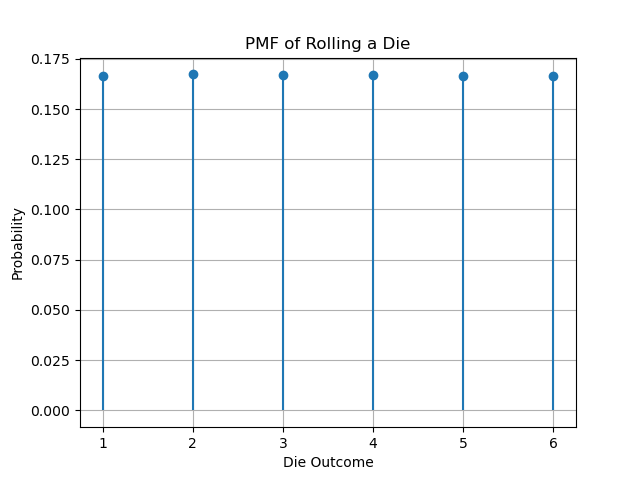
\includegraphics[width=\columnwidth]{figs/Figure_1.png}
\end{figure}
\end{document}
